\section{Git remotes}
\begin{frame}[fragile]
  \slidetitle
  This section covers the following topics:
  \begin{itemize}
    \item Git protocols
    \item Git remote repository concept
    \item Add remote repositories
    \item Synchronize with remote repositories
  \end{itemize}
\end{frame}

\subsection{Git protocols}
\begin{frame}[fragile]
  \subslidetitle
  Git repositories can be accessed locally or over the network.
  \\
  \vspace{1em}
  Various protocols are supported:
  \begin{itemize}
  \opt{local}  {file system based}
  \opt{http[s]}{good for read only access without password}
  \opt{ssh}    {normally used for read-write access}
  \opt{git}    {git native protocol on port 9418}
  \opt{legacy} {ftp, rsync, ...}
  \end{itemize}
  \vspace{1em}
  %With ssh configured we are not prompt for our password on every request
  SSH provides us the possibility to authenticate without having to enter the password on every request.
\end{frame}

\subsection{Remote repositories}
\begin{frame}[fragile]
  \subslidetitle
  The \cmd{git remote} allows to manage remote repositories:
  \begin{lstlisting}
$ (*\textcolor[HTML]{0000AA}{git remote show}*)
origin

$ (*\textcolor[HTML]{0000AA}{git remote show origin}*)
* remote origin
  Fetch URL: https://github.com/segfault-trainings/gitmoon.git
  Push  URL: https://github.com/segfault-trainings/gitmoon.git
  HEAD branch: master
  Remote branch:
    master tracked
  Local branch configured for 'git pull':
    master merges with remote master
  Local ref configured for 'git push':
    master pushes to master (up to date)
\end{lstlisting}
  \vspace{1em}
  Note: the default remote is called \textbf{origin}
\end{frame}

\subsection{Remote commands}
\begin{frame}[fragile]
  \subslidetitle
  The following commands operate on remote repositories:
  \begin{itemize}
    \item \cmd{git fetch [remote]} \\
      Downloads all branches from another repository
    \item \cmd{git pull [remote] [branch]} \\
      Does a {\bf fetch} and then {\bf merges} the remote branch into the current branch
    \item \cmd{git pull --rebase [remote] [branch]} \\
      Does a {\bf fetch} and then {\bf rebases} the current branch on top of the remote branch
    \item \cmd{git remote update} \\
      Does a {\bf fetch} for all remotes
    \item \cmd{git push [remote] [branch]} \\
      Pushes commits/branches to a remote
  \end{itemize}
\end{frame}

\subsection{Example: Adding a remote repository}
\begin{frame}[fragile]
  \subslidetitle
  This example adds a repository as remote called \textbf{upstream}:
  \begin{lstlisting}
$ (*\textcolor[HTML]{0000AA}{git remote add upstream} \textcolor[HTML]{444444}{URL}*)
$ (*\textcolor[HTML]{0000AA}{git remote show}*)
origin
upstream
\end{lstlisting}
\vspace{1em}
\cmd{URL} needs to be replaced with the URL of the remote repository
\vspace{1em}
\center 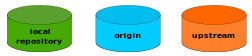
\includegraphics{diagrams/remote-add.pdf}
\end{frame}

\subsection{Example: Pushing commits to a remote}
\begin{frame}[fragile]
  \subslidetitle
  This example pushes the local master branch to the \textbf{upstream} remote:
  \begin{lstlisting}
$ (*\textcolor[HTML]{0000AA}{git push upstream master}*)
git push upstream master
Counting objects: 6, done.
Delta compression using up to 2 threads.
Compressing objects: 100% (6/6), done.
Writing objects: 100% (6/6), 331.07 KiB | 0 bytes/s, done.
Total 6 (delta 0), reused 0 (delta 0)
remote: ...
To (*\textcolor[HTML]{444444}{URL}*)
 * [new branch]      master -> master
\end{lstlisting}
\vspace{-1.1em}
\center 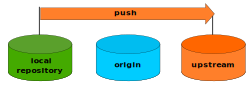
\includegraphics{diagrams/remote-push.pdf}
\end{frame}

\subsection{Example: Pulling commits from a remote}
\begin{frame}[fragile]
  \subslidetitle
  This example updates the local master branch with the origin master branch:
  \begin{lstlisting}
$ (*\textcolor[HTML]{0000AA}{git pull}*)
remote: Counting objects: 6, done.
remote: Compressing objects: 100% (6/6), done.
remote: Total 6 (delta 0), reused 0 (delta 0)
Unpacking objects: 100% (6/6), done.
From (*\textcolor[HTML]{444444}{URL/mygitmoon.git}*)
 * [new branch]      master     -> origin/master
\end{lstlisting}
\center 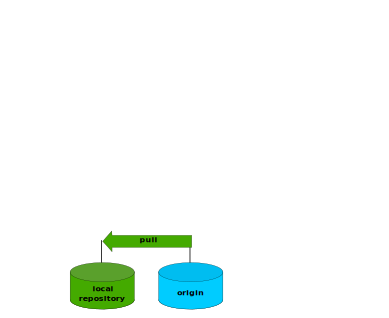
\includegraphics{diagrams/remote-pull.pdf}
\end{frame}

\subsection{Example: Checkout a remote branch}
\begin{frame}[fragile]
  \subslidetitle
  In order to work on a remote branch we are checking out a local branch tracking the remote branch.

  \begin{lstlisting}
(*\textcolor[HTML]{18B2B2}{(master)}*) $ (*\textcolor[HTML]{0000AA}{git checkout -b fix-title origin/fix-title --track}*)
Branch fix-title set up to track remote branch fix-title from origin.
Switched to a new branch 'fix-title'
\end{lstlisting}
  \vspace{1em}
  Now we can use \cmd{git push} and \cmd{git pull} to synchronize these branches.

  \vspace{1em}
  Note: Git does automatically setup the master branch to track the remote master branch.
\end{frame}

\subsection{Git appliances}
\begin{frame}[fragile]
  \subslidetitle
  There are various git appliances, providing the following features:
  \begin{itemize}
    \item Forking a repository
    \item Creating pull requests
    \item Offers branching models
  \end{itemize}
\end{frame}

\subsection{Configure SSH access}
\begin{frame}[fragile]
  \subslidetitle
  Create a SSH key pair:
  \begin{lstlisting}
$ (*\textcolor[HTML]{0000AA}{ssh-keygen -f \textasciitilde/.ssh/id\_rsa\_workshop}*)
Generating public/private rsa key pair.
Enter passphrase (empty for no passphrase): (*\textcolor[HTML]{0000AA}{<enter>}*)
Enter same passphrase again: (*\textcolor[HTML]{0000AA}{<enter>}*)
Your identification has been saved in .../.ssh/id_rsa_workshop.
Your public key has been saved in .../.ssh/id_rsa_workshop.pub.
The key fingerprint is:
7e:f8:15:2a:b3:a2:9c:30:4e:c7:60:50:a4:d5:a9:82 user@host
The key's randomart image is:
+--[ RSA 2048]----+
|   . . .         |
|  . = = S        |
|   = X * X O o   |
...
\end{lstlisting}
\end{frame}

\subsection{Configure SSH access}
\begin{frame}[fragile]
  \subslidetitle
  Display your public key:
  \begin{lstlisting}
$ (*\textcolor[HTML]{0000AA}{cat \textasciitilde/.ssh/id\_rsa\_workshop.pub}*)
ssh-rsa AAAAB3NzaC1yc2EAAAADAQABAAABAQDOmt7Y4H51gc2m
GmZsFzES6shVLFLEJ/lFCTwyosWHYDaluK71nGCelp61oTocgf4N
HBwTZmo0EZ1k0RHYt8Q3LF8e5fbC+dXt5E35XtkVFuUC7IG2/6fm
NW41j3lw9UUVrOBDgx+QvvoCuRQaxNd4mRaLsRbj9WXt17hGuNNW
ioKPWLSpw/4KHJ34hCrnliAQJ+jlW/0ieOooFp057diCka6Jn7BW
jXHi8sWMxIfyPyV2+4Kt8OpChFNYjzaL5LMRRhMnvJ8zP5SFJB2q
HP50zPYQ+gKoSda7GZedZRgD7gT7ir/u8X9HSpNyTNTafhp9+3Aj
uUiYLTgtczTgYk/T user@host
\end{lstlisting}

  This whole output can be added to the SSH access keys
  section in the web frontend of your git appliance.
\end{frame}

\subsection{Exercises}
\begin{frame}[fragile]
  \subslidetitle
  \begin{exercise}
    \item Create a SSH key pair as shown in the slides
    \item Configure SSH access in your git appliance
    \item Clone the new repository in your home (repository given by instructor)\\
      \cmd{cd} first to switch to your home directory, then\\
      \cmd{git clone URL newgitmoon}
    \item Implement features given by instructor in new branch
    \item Push branch
  \end{exercise}
\end{frame}

\subsection{Workflows / Branching Models}
\begin{frame}[fragile]
  \subslidetitle
  Centralized Workflow
  \center 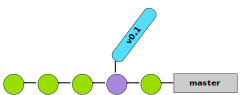
\includegraphics{diagrams/git-centralized-workflow.pdf}

  \vspace{2em}
  \begin{itemize}
    \item Only the \lstinline{master} branch is used
    \item First rebase, then push
    \item Often used to transition from old-ish VCS
  \end{itemize}
\end{frame}

\subsection{Workflows / Branching Models}
\begin{frame}[fragile]
  \subslidetitle
  Feature Branch Workflow
  \center 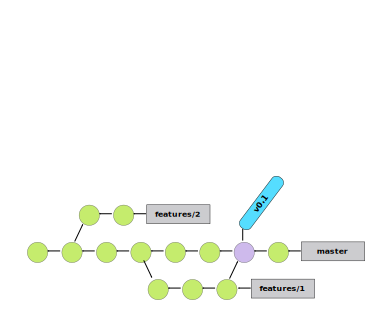
\includegraphics{diagrams/git-workflow.pdf}

  \vspace{2em}
  \begin{itemize}
    \item Development in small feature branches
    \item Chance for Pull Requests
    \item No broken code on \lstinline{master}
  \end{itemize}
\end{frame}

\subsection{Workflows / Branching Models}
\begin{frame}[fragile]
  \subslidetitle
  Gitflow Workflow
  \center 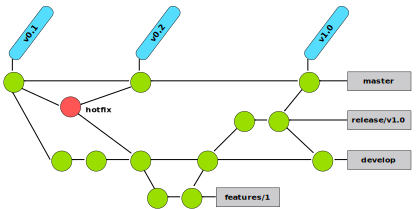
\includegraphics[width=\textwidth]{diagrams/git-gitflow-workflow.pdf}

  \begin{itemize}
    \item Like \textit{Feature Branch Workflow}
    \item Assign special roles to certain branches
  \end{itemize}

\end{frame}

\subsection{Workflows / Branching Models}
\begin{frame}[fragile]
  \subslidetitle
  Forking Workflow
  \center 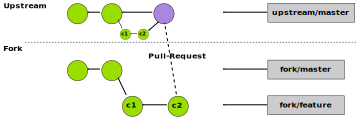
\includegraphics{diagrams/git-forking-workflow.pdf}

  \vspace{2em}
  \begin{itemize}
    \item Every contributor has it's own copy (fork) of the repo
    \item Contribute with Pull Requests
    \item Most often used in Open Source
  \end{itemize}

\end{frame}
